\begin{tikzpicture}[x=1cm,y=1cm,>=stealth,font=\small]
\path[use as bounding box] (-3,-2.5) rectangle (5.1,4.6);
\draw[->,gray] (-2.8,0)--(4.8,0) node[right] {$x$};
\draw[->,gray] (0,-2.2)--(0,4.2) node[above] {$y$};
\node[below left] at (0,0) {$O$};
\draw[blue,thick,domain=-2.5:4,samples=90] plot (\x,{\x*\x/4});
\node[blue,right] at (3.8,3.5) {$x^2=4y$};
\draw[orange,thick] (-2.4,1.4)--(1.4,-2.4) (.8,-2.4)--(4,4);
\draw[gray,thick] (-2,1)--(4,4);
\draw[red,very thick] (1,-2)--(1,2.5);
\fill (-2,1) circle (2pt) node[below left=3pt] {$A(-2,1)$};
\fill (4,4) circle (2pt) node[above left] {$B(4,4)$};
\fill[red] (1,-2) circle (2pt) node[right] {$M(1,-2)$};
\fill[red] (1,2.5) circle (2pt) node[above left] {$N(1,\tfrac52)$};
\node[red,right,fill=white,inner sep=3pt] at (1,.7) {$x_M=x_N=1$};
\end{tikzpicture}
